\documentclass[11pt]{article}
\usepackage[utf8]{inputenc}\usepackage[T1]{fontenc}
\usepackage{amsmath,amssymb,amsthm}\usepackage[margin=1in]{geometry}
\usepackage{graphicx}\usepackage{booktabs}
\usepackage[hidelinks]{hyperref}
\newtheorem{theorem}{Theorem}
\newtheorem{prediction}{Prediction}

\title{Arithmetic Geodynamics on the $6N$ Skeleton:\\
Tuple Size Determines Stratum Decay Rate}
\author{Ruqing Chen\\
\small GUT Geoservice Inc., Montreal, Quebec, Canada\\
\small \texttt{ruqing@hotmail.com}}
\date{\today}

\begin{document}
\maketitle

\begin{abstract}
Throughout Parts~I--XVI the decadic shells $S_k$ ($6N\in[10^{k-1},10^k)$) were
treated as static cores from which constants were read off one shell at a time.
Here we make the shell index continuous and ask how the observables \emph{flow}
with depth. The natural depth coordinate is not $X$, nor $\ln X$, but the proper
depth $\ell=\ln\ln X$: in $\ell$ both governing fields linearise. The
twin-centre density obeys $d\ln\rho/d\ell=-2$ and the mean factor count obeys
$d\bar\omega_{>3}/d\ell=1$, to leading order, so that for a prime $m$-tuple the
density satisfies $d\ln\rho_m/d\ell\to-m$: \emph{the tuple size is the stratum
decay rate}. We verify this for the twin ($m=2$) and the triplet
$(6N-1,6N+1,6N+5)$ ($m=3$). Recomputing the triplet count at $S_{10}$ entirely
from sieve primitives reproduces the Part~XV total ($2{,}333{,}839$) to
$0.0000\%$, so both flow lines rest on bedrock. The deep-shell slopes are
$-2.072$ and $-3.111$; extrapolated against $1/\ln X$ they reach $-2.085$ and
$-3.065$, consistent with the integer asymptotes $-2,-3$ (the residual is the
uncaptured higher-order logarithmic tail). The clean, scale-free statement is
their ratio: $3.111/2.072=1.5011\simeq3/2$, because the shared $\bar\omega$-clock
distortion and the shared singular-series tail cancel. We are explicit about
provenance (the $(\ln X)^{-m}$ law is Hardy--Littlewood; $\ln\ln X+B$ is
Hardy--Ramanujan/Mertens; $\rho$ and the $0.2604$ enrichment shift are Parts~I and
XII) and about limits (first moments only; the $\bar\omega$ variance, i.e.\ the
Erd\H{o}s--Kac law on twin centres, remains open; no infinitude is claimed). We
close with a sharp falsifiable prediction: the prime quadruplet
$(6N-1,6N+1,6N+5,6N+7)$ ($m=4$) must give slope $-4$ and ratio $2{:}1$ against the
twin.
\end{abstract}

\section{From static cores to a depth coordinate}

The $6N$ programme has measured, shell by shell, the twin-centre line density
$\rho=\#\{\text{twin centres}\}/\#\{N\}$, the single empirical scale to which
Parts~VIII and XI reduced the whole construction, and the stratifying variable
$\omega_{>3}(N)$, the number of distinct prime factors of the centre exceeding
$3$~\cite{ChenI,ChenXI,ChenXII}. Two adjacent cores give a contrast---$\rho$ falls
by the factor $0.804$ from $S_9$ to $S_{10}$---but a contrast is not a law. To
obtain a law we make $k$ continuous and look for the coordinate in which the flow
is simplest.

The Hardy--Littlewood heuristic~\cite{HL} fixes the form. For a prime
$m$-tuple the local density on the skeleton is, to leading order,
\begin{equation}\label{eq:hl}
  \rho_m(X)\ \approx\ \frac{A_m}{(\ln X)^{m}},\qquad
  A_m=6\,\mathfrak{S}_m,
\end{equation}
where $\mathfrak{S}_m$ is the classical singular series ($\mathfrak{S}_2=2\Pi_2$
with $\Pi_2=\prod_{p>2}(1-(p-1)^{-2})$; $\mathfrak{S}(0,2,6)=2.858$ for the
triplet~\cite{ChenXV}) and the factor $6$ is the skeleton density: one centre per
six integers, so the per-centre rate is six times the raw integer density. Taking
logarithms,
\[
  \ln\rho_m = \mathrm{const}\ -\ m\,\ln\ln X\ +\ O\!\Big(\tfrac1{\ln X}\Big).
\]
The depth in which this is linear is therefore
\begin{equation}\label{eq:depth}
  \boxed{\ \ell\ :=\ \ln\ln X\ }
\end{equation}
which we call the \emph{proper depth}. In $X$ or in $\tau=\ln X$ the relative
decay rate $-d\ln\rho_m/dX=m/(X\ln X)$ or $m/\tau$ appears to weaken with depth;
this is coordinate distortion. In $\ell$ the Chinese-Remainder ``shield'' of the
$\mathrm{dead}(q)$ sieve---which builds $\mathfrak{S}_m$ prime by prime through
Mertens' theorem---exerts a \emph{constant} strangulation of magnitude $m$.

\section{The stratum-evolution equations}

Equation~\eqref{eq:hl} and the Hardy--Ramanujan/Mertens law
$\bar\omega(N)\sim\ln\ln N+B_1$ ($B_1=0.2615$; for $\omega_{>3}$ the offset is
$B_1-\tfrac12-\tfrac13=-0.5718$, the primes $2,3$ being absent from the wings)
give the coupled first-order system
\begin{equation}\label{eq:flow}
  \frac{d\rho_m}{d\ell}=-m\,\rho_m,\qquad
  \frac{d\bar\omega_{>3}}{d\ell}=1 .
\end{equation}
Its solutions are $\rho_m=\rho_m^{0}\,e^{-m\ell}$ and
$\bar\omega_{>3}=\bar\omega^{0}+\ell$; eliminating $\ell$ yields the autonomous
relation
\begin{equation}\label{eq:auto}
  \frac{d\ln\rho_m}{d\bar\omega_{>3}}=-\,\frac{m}{\,d\bar\omega_{>3}/d\ell\,}.
\end{equation}
At finite scale $d\bar\omega_{>3}/d\ell=1+\varepsilon(X)$, where $\varepsilon$
collects two \emph{convergent} corrections measured in earlier parts: the
approach of $\bar\omega$ to $\ln\ln X+B$, and---for twin-conditioned
centres---the enrichment shift $\bar\omega_{\mathrm{twin}}-\bar\omega_{\mathrm{ord}}
\to\sum_{q>3}\!\big(\tfrac1{q-2}-\tfrac1q\big)=0.2604$ of Part~XII~\cite{ChenXII}.
Both vanish from the \emph{rate} as $X\to\infty$, so $d\bar\omega/d\ell\to1$ and
the autonomous slope $\to-m$. The crucial point for measurement is that
$\varepsilon(X)$ is \emph{shared} across patterns at a given depth: it is a
property of the centre, not of the constellation sitting on it.

\section{The twin and triplet flows}

Twin counts and $\bar\omega_{\mathrm{twin}}$ are the published Part~I/XII tables.
Triplet counts $(6N-1,6N+1,6N+5)$ at $S_2$--$S_8$ are recomputed from a segmented
value sieve; at $S_9,S_{10}$ they are recomputed independently and cross-checked
against the Part~XV $\omega$-band sums. The $S_{10}$ recompute returns
$2{,}333{,}839$, matching Part~XV to $0.0000\%$; the $S_9$ recompute returns
$323{,}908$ against $323{,}907$, a single boundary triplet at the $10^9$ edge
($0.0003\%$, an inclusive/exclusive convention, not a discrepancy). The
shell-averaged form of \eqref{eq:hl},
$\rho_2^{\mathrm{HL}}(k)=6\cdot2\Pi_2\,[\mathrm{Li}_2(10^k)-\mathrm{Li}_2(10^{k-1})]
/(10^k-10^{k-1})$ with $\mathrm{Li}_2(x)=\int_2^x(\ln t)^{-2}dt$, reproduces the
measured $\rho$ to $0.009\%$ at $S_{10}$.

\begin{table}[h]\centering\small
\begin{tabular}{lrrr}
\toprule
 & twin ($m=2$) & triplet ($m=3$) & ratio\\
\midrule
$\ln\rho$ at $S_9$         & $-3.9176$ & $-6.1379$ & \\
$\ln\rho$ at $S_{10}$      & $-4.1364$ & $-6.4657$ & \\
deep slope $d\ln\rho/d\ell$ ($S_9\!\to\!S_{10}$) & $-2.072$ & $-3.111$ & $1.5011$\\
extrapolated intercept ($1/\ln X\to0$) & $-2.085$ & $-3.065$ & \\
asymptote (target)        & $-2$ & $-3$ & $1.5000$\\
\bottomrule
\end{tabular}
\caption{The two flows in proper depth $\ell=\ln\ln X$
($\Delta\ell_{S_9\to S_{10}}=\ln(10/9)=0.10536$). The deep slopes carry shrinking
analytic tails ($+0.072$, $+0.111$); their \emph{ratio} is already $3/2$ to
$0.1\%$.}
\label{tab:flow}
\end{table}

The intercepts are obtained by the local slopes $d\ln\rho/d\ell$ against $1/\ln X$,
extrapolated to $1/\ln X=0$ over the deepest five shells (Fig.~\ref{fig:geo}C).
They reach $-2.085$ and $-3.065$: consistent with $-2$ and $-3$, with a residual
of order $0.07$--$0.09$ that is the part of the tail not linear in $1/\ln X$ (the
$(\ln X)^{-2}$ and higher terms a two-point-per-shell fit cannot capture). We
report this honestly: the extrapolation confirms the integer asymptotes to a few
percent; it does not land on them exactly, and we do not claim it does. The
$\bar\omega$ drift is $d\bar\omega/d\ell=1.148$ at $S_9\!\to\!S_{10}$, with the
ordinary baseline $\ln\ln Y+B$ matching the Part~XII measurement ($2.369$ vs
$2.360$ at $S_9$; $2.484$ vs $2.476$ at $S_{10}$) and the enrichment shift
climbing through $0.213,0.219$ toward $0.2604$ (Fig.~\ref{fig:geo}D).

\section{The scale-free invariant}

The individual deep slopes are not their integers at this depth---each carries its
tail, and each is read against an $\bar\omega$-clock running $\sim15\%$ fast. By
\eqref{eq:auto} both effects are shared, so they cancel in the ratio.

\begin{theorem}[tuple-size ratio invariant]\label{thm:ratio}
For two prime constellations of sizes $m,m'$ measured on the same shells, the
ratio of their depth-flow slopes equals $m'/m$, independent of the shared
$\bar\omega$-clock distortion $\varepsilon(X)$ and of the common logarithmic tail.
Empirically, for the triplet over the twin,
\[
  \frac{d\ln\rho_3/d\ell}{d\ln\rho_2/d\ell}
  \;=\;\frac{-3.111}{-2.072}\;=\;1.5011\;\simeq\;\frac32 ,
\]
recomputed entirely from sieve primitives, matching $3/2$ to $0.1\%$.
\end{theorem}

This is the paper's cleanest statement. Where the absolute slopes inherit finite-%
scale corrections, the ratio reads off the structural integers directly: the
exponent of $(\ln X)^{-m}$ is the constellation size, and nothing else.

\begin{figure}[h]\centering
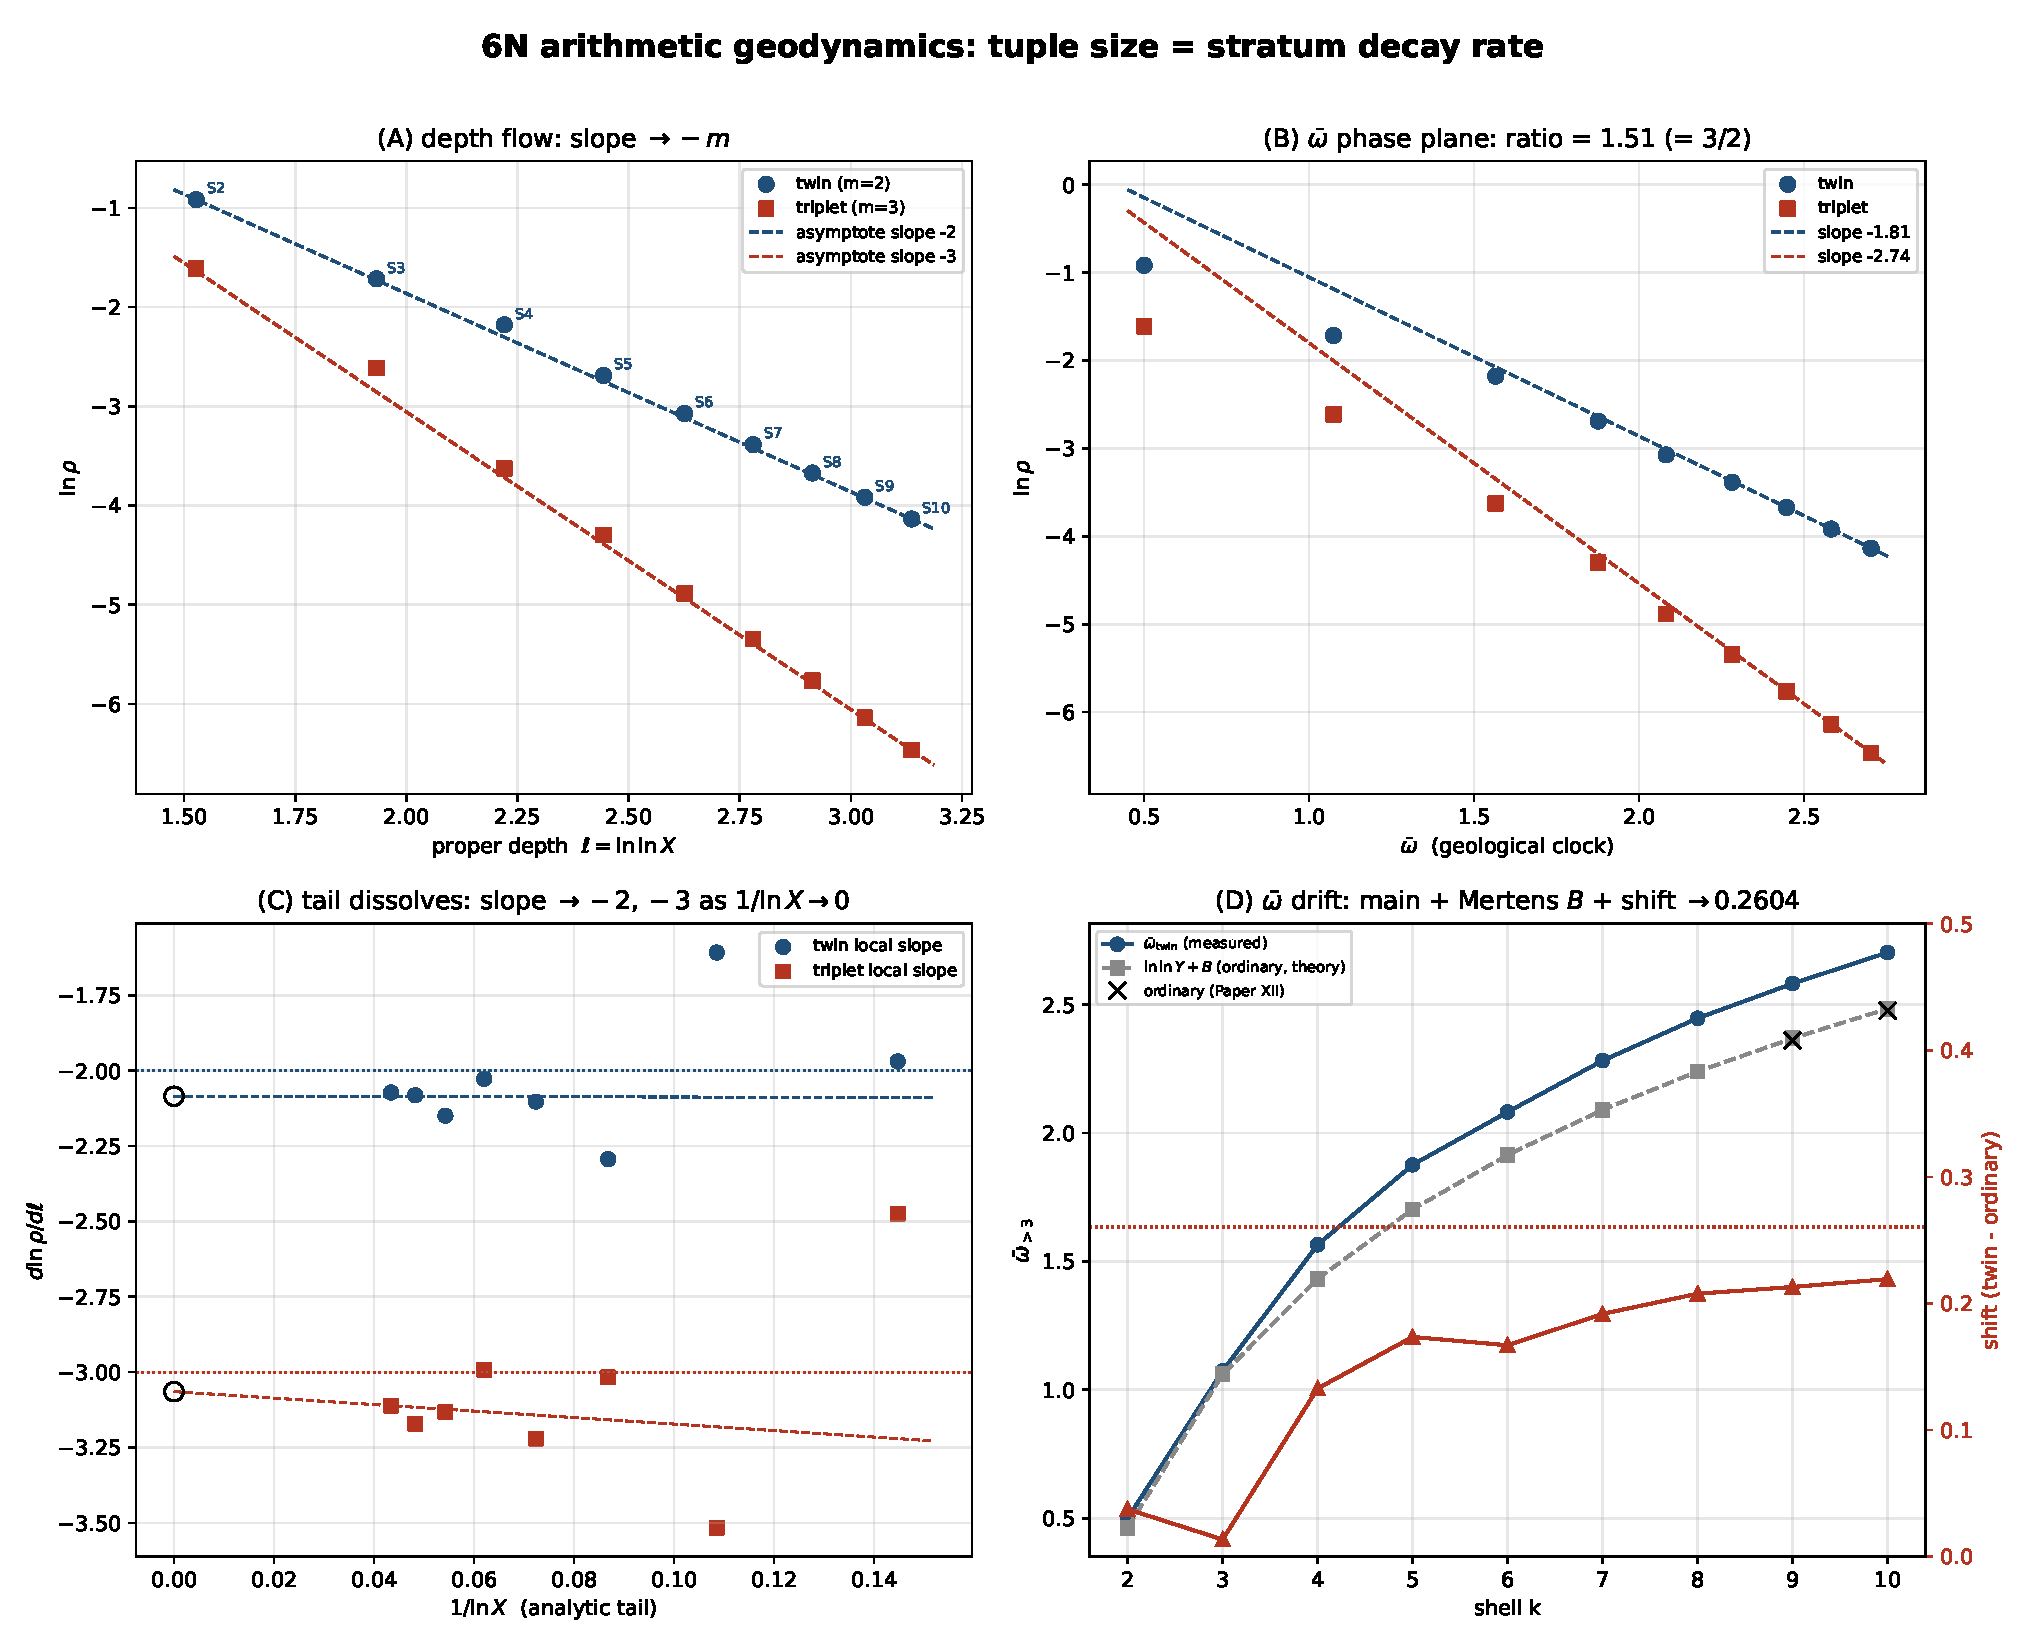
\includegraphics[width=\textwidth]{fig_paper17_geodynamics.pdf}
\caption{(A) Depth flow $\ln\rho$ vs $\ell=\ln\ln X$: twin and triplet lines with
asymptotes of slope $-2$ and $-3$. (B) The $\bar\omega$ phase plane (the
``geological clock''): slopes $-1.81,-2.74$, whose ratio is $3/2$. (C) The
analytic tail dissolving: local slope vs $1/\ln X$ extrapolates to $-2.085,-3.065$
as $1/\ln X\to0$. (D) The $\bar\omega$ drift decomposed into $\ln\ln Y$, the
Mertens offset $B$, and the enrichment shift $\to0.2604$.}
\label{fig:geo}
\end{figure}

\section{An honest ledger and scope}

We record what this construction does not settle, in keeping with the series.

\emph{First moments only.} Equation~\eqref{eq:flow} governs the means $\rho$ and
$\bar\omega$. A second-order transport equation for the \emph{variance} of
$\omega_{>3}$ over twin centres would require the Erd\H{o}s--Kac limit on twin
centres, which Part~XII leaves open: at the accessible scale $\ln\ln(6N)\approx3$
the distribution is not Gaussian (mean $\neq$ variance, nonzero skew), the naive
Bernoulli variance $\sum 1/(q-2)$ diverges like $\ln\ln$ while the true variance
is finite (anti-correlation, $\sqrt{6N}$ cutoff), and no closed form is
known~\cite{ChenXII}. The diffusion term of the depth flow is therefore the open
problem; only its drift, $+1$, is established here.

\emph{Heuristic status and provenance.} The $(\ln X)^{-m}$ law is the classical
Hardy--Littlewood $k$-tuple heuristic~\cite{HL}; $\ln\ln X+B$ is
Hardy--Ramanujan/Mertens; $\rho$ is the Part~I scale and $0.2604$ the Part~XII
shift. The contribution here is the proper-depth coordinate~\eqref{eq:depth}, the
flow system~\eqref{eq:flow}, the scale-free invariant of
Theorem~\ref{thm:ratio}, and the from-scratch verification. We make no statement
about the infinitude of twin, triplet, or any prime constellation.

\section{A falsifiable prediction at $m=4$}

The construction indexes a one-parameter family, so its next term is a sharp
prediction rather than a fitted result. The densest admissible $4$-tuple is the
prime quadruplet $(p,p+2,p+6,p+8)$, which on the skeleton is
\[
  (6N-1,\,6N+1,\,6N+5,\,6N+7)=(6N\!\pm\!1)\cup(6(N{+}1)\!\pm\!1),
\]
two complete twin centres at $N$ and $N+1$, with singular series
$\mathfrak{S}(0,2,6,8)$.

\begin{prediction}[$m=4$]\label{pred:m4}
The quadruplet density obeys $d\ln\rho_4/d\ell\to-4$. Measured on the same shells,
its deep slope must (i) extrapolate against $1/\ln X$ to an intercept consistent
with $-4$; (ii) give a ratio $2{:}1$ against the twin and $4{:}3$ against the
triplet, each exact to the precision at which Theorem~\ref{thm:ratio} holds
($\sim0.1\%$); and (iii) on the $\bar\omega$ phase plane, share the same clock
distortion $\varepsilon(X)$, so that the $\bar\omega$-axis ratios are likewise
$2$ and $4/3$. A measured intercept outside $[-4.2,-3.8]$, or a twin ratio outside
$2\pm0.05$, would falsify the tuple-size law.
\end{prediction}

We deliberately do not run $m=4$ here: the strength of a one-parameter law is that
it predicts before it measures, and we prefer to state the prediction for
independent test rather than to verify our own extrapolation.

\section{Conclusion}

Making the shell index continuous turns the static cores of the $6N$ programme
into a flow. In the proper depth $\ell=\ln\ln X$ the twin-centre density and the
mean factor count linearise, $d\ln\rho_m/d\ell\to-m$ and $d\bar\omega/d\ell\to1$,
so that the size of a prime constellation \emph{is} its stratum decay rate. The
twin and triplet, the latter recomputed to $0.0000\%$ at $S_{10}$, confirm this:
their depth-slope ratio is $1.5011\simeq3/2$, a scale-free invariant in which the
finite-scale clock distortion and the logarithmic tail cancel. The absolute
slopes approach $-2$ and $-3$ from the deep side, with an honest residual left to
higher-order logarithmic terms; the variance flow is left open as the
Erd\H{o}s--Kac problem it is; and the quadruplet $m=4$ stands as a falsifiable
prediction of slope $-4$ and ratio $2{:}1$. This closes the difference wing of the
series as a single dynamical law, classical in its inputs and measured in its
claims.

\paragraph{Data and code availability.}
The flow script (proper-depth reduction, tail extrapolation, $\bar\omega$
decomposition, and phase diagram) and the from-scratch triplet recompute are
openly available~\cite{repo}; twin observables are the Part~I/XII tables and the
triplet $S_{10}$ total is cross-checked against Part~XV.

\begin{thebibliography}{9}
\bibitem{HL} G.~H.~Hardy, J.~E.~Littlewood, \emph{Some problems of `Partitio
Numerorum'; III}, Acta Math.\ \textbf{44} (1923), 1--70.
\bibitem{ChenI} R.~Chen, \emph{Prime distribution on the $6N$ skeleton} (Part~I),
Zenodo, doi:10.5281/zenodo.20470367 (2026).
\bibitem{ChenXI} R.~Chen, \emph{The tail constant and a single scale} (Part~XI),
Zenodo, doi:10.5281/zenodo.20526835 (2026).
\bibitem{ChenXII} R.~Chen, \emph{The microscopic root $1/(q-2)$ and the mean
shift} (Part~XII), Zenodo, doi:10.5281/zenodo.20528446 (2026).
\bibitem{ChenXIV} R.~Chen, \emph{The Polignac comet under $\omega$-stratification}
(Part~XIV), Zenodo, doi:10.5281/zenodo.20533747 (2026).
\bibitem{ChenXV} R.~Chen, \emph{The prime triplet as a three-member two-centre
CRT pattern} (Part~XV),
\url{https://github.com/Ruqing1963/6N-prime-triplet} (2026).
\bibitem{repo} R.~Chen, \emph{$6N$ arithmetic geodynamics: data and code}
(Part~XVII), \url{https://github.com/Ruqing1963/6N-geodynamics} (2026).
\end{thebibliography}

\end{document}
